\chapter{Cyberbullying Analysis}


This section presents our data-driven analysis of cyberbullying on 7cot. While 7cot and other emotional support systems are successful, their members and the listeners on such sites are especially vulnerable targets for cyberbullies. Members, who are already visiting to address an emotional need due to a distress would be taken to even more serious levels of stress and depression by a listener who cyberbullies. When listeners are exposed to cyberbullying, it is not only the health of the user that suffers, but also the health of the entire platform. This is because listeners who are harassed by nefarious members may suddenly become demotivated to participate on the site and opt to no longer volunteer their time or service. This loss of listeners, who are in most ways the lifeblood of a strong emotional support system, may have long term, possibly even fatal effects on the viability of the platform. It is therefore, important to begin to unearth information about the nature of cyberbullying on emotional support platforms, and in particular, to learn about the extent to which harassment occurs, the effects of this harassment on users and on the platform, and whether basic methods to curtail harassment are effective. The analysis is anchored around two important research questions :

1. Is cyberbullying prevalent on an emotional support service? If so, what broad types of cyberbullying are occurring?

2. Does the act of blocking a bully from conversing with another change their negative behaviors?

While there is support in the research literature and popular press that cyberbullying is present, the levels to which they are prevalent in a social system has not been explored from a data driven perspective. Finally, checking if and how interventions widely adopted in social systems, such as electing to ‘block’ someone, has an effect on the behavior of cyberbullies help us evaluate if new safeguards are even necessary. While previous studies on cyberbullying focuses on the effects of the practice on individual victims or even on the offenders of cyberbullying, which is an extremely worthy endeavor ~\cite{hinduja2010bullying}. Our study takes the unique perspective of exploring the effect of cyberbullying on the overall health and viability of the online social system itself. We do so by evaluating how listeners may be bullied and discouraged from participating in the service by members.

\section {How Much and What Kinds of Cyberbullying Exist ?}

\begin{figure}
	\centering
	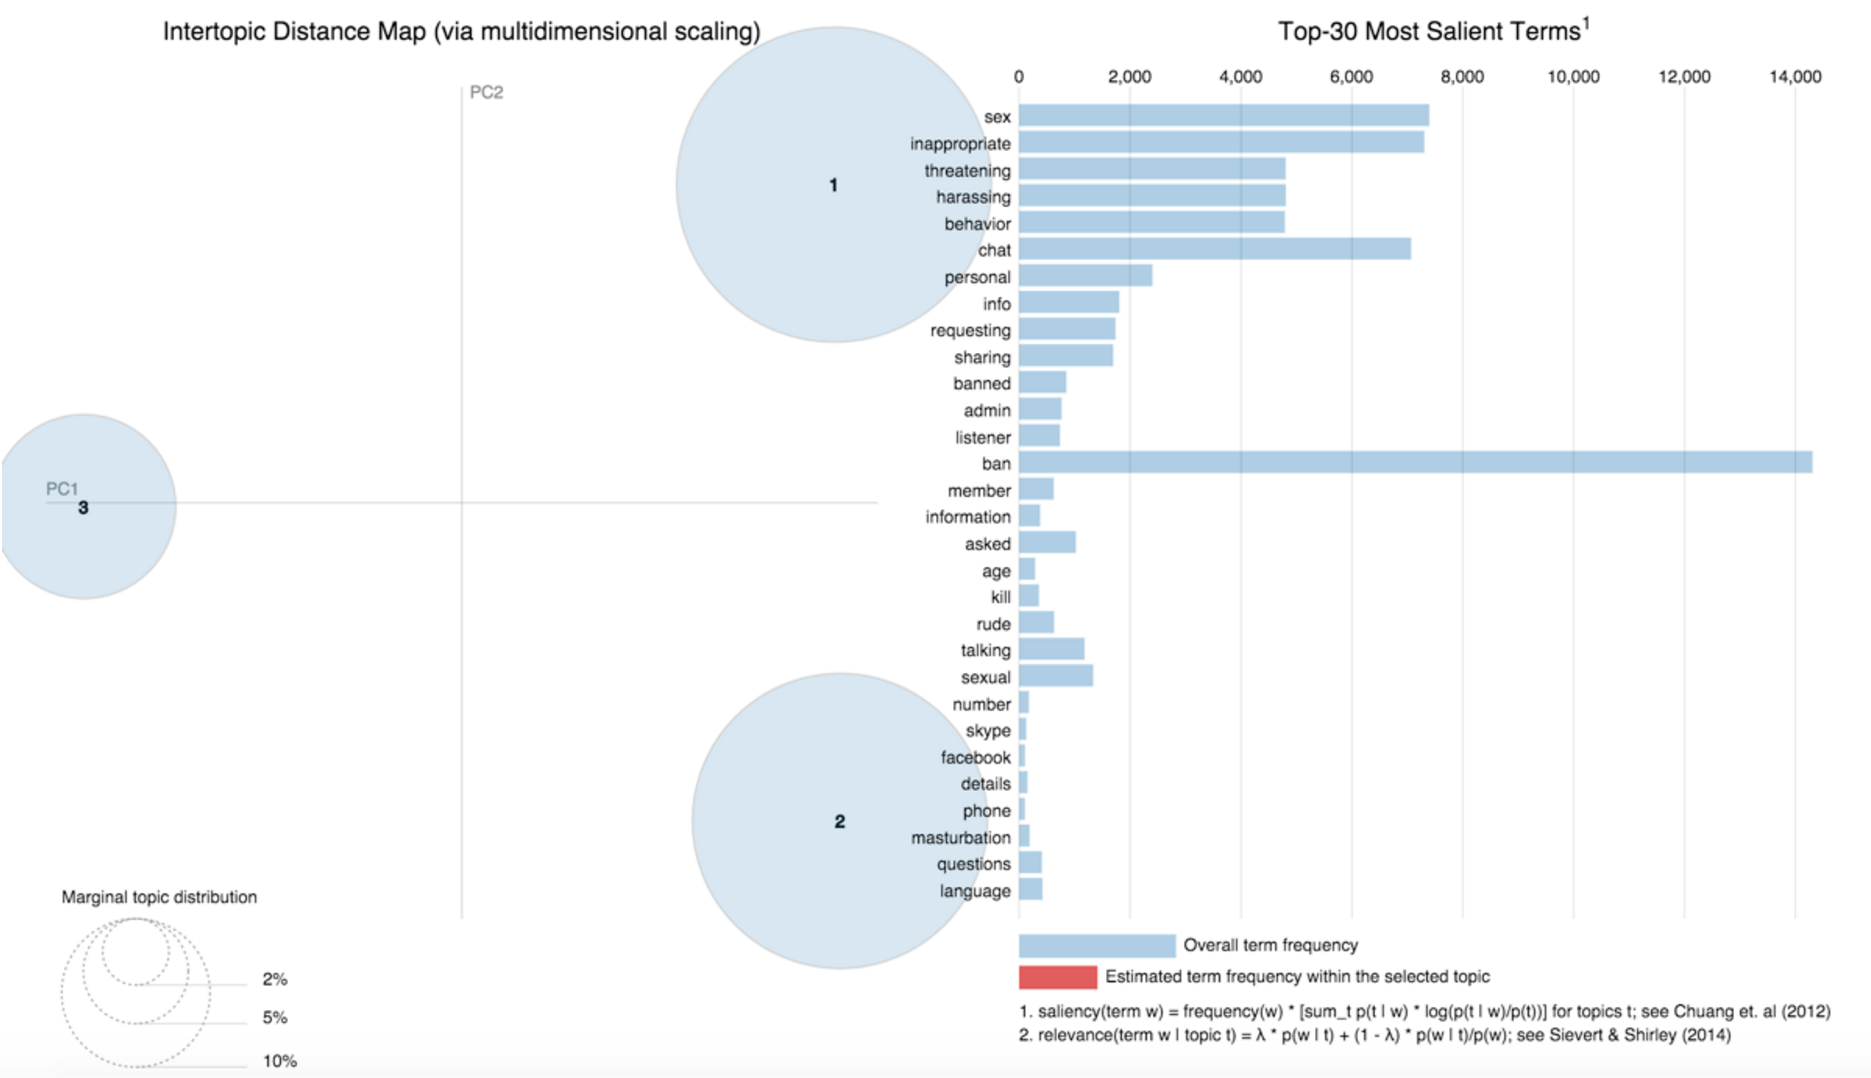
\includegraphics[width=4in5]{LDAVIS.png}
	\caption{Intertopic map of LDAVIS clusters}
	\label{fig:topicmap}
\end{figure}

We first examine the degree and ways in which harassment occurs on 7cot. Each 7cot listener has the opportunity to ‘block’ a member from communicating with them in a one-on-one conversation on the site. We postulate that block events only occur if a member bullies a listener during such a conversation. This is because members and listeners can only communicate one-on-one through conversations and because blocks can only be applied in the conversation interface. When a listener elects to block a member, he/she is allowed to enter a ‘note’ as to why the block is applied. 7cot administrators regularly review these notes to identify members that should be banned from the site for constantly bullying others.

\begin{table}
	\centering
	\begin{tabular}{|c c c|} 
		\hline
		Users & Count & Percentage \\ 
		\hline\hline
		Num. Members & 452,605 & - \\ 
		Num. Listeners & 169,372 & -  \\
		Conversations &   3.2 M & - \\
		Cyberbully Members & 19,281 & 4.26\% \\
		Listeners exposed to a cyberbully & 37,262 & 22\% \\
		\hline
	\end{tabular}
	\caption{Summary of Users and Cyberbullies}
	\label{table:1}
\end{table}

Table ~\ref{table:1} provides a summary of the volume of members and listeners who are or were exposed to a cyberbully. For this table, we define a cyberbully as an individual who was either blocked by at least one listener in a one-on-one conversation. We identify a total of 19,281 members who were either blocked or banned during this time period, representing 4.26\% of all members on the site. While this percentage appears to be small, these 4.26\% of members actually held a one-on-one conversation with 37,262, or 22\%, of all listeners on 7cot. Thus, even though a small number of members may have performed an action that led to a block or a ban but they run the risk of exposing a large proportion of listeners to emotionally damaging behaviors.

Notes left by listeners when they elect to block a member provides some insight into how and why a listener may have been harassed by the cyber- bully. We employ an extension of Latent Dirichilet Allocation (LDA) ~\cite{blei2003latent} called LDAVIS ~\cite{sievert2014ldavis}. LDA is a learning algorithm that partitions documents in a corpus into clusters, with clustered documents containing a similar distribution of words. Evaluation of the words in the cluster are thus suggestive of a latent topic or theme in the documents. LDAVIS extends LDA by choosing to filter away words that appear across a number of topic clusters based on a measure of the relevance of a term to a topic. The relevance of a term to a particular topic is calculated by adding two quantities. The first quantity is the probability of a term under a particular topic and the second quantity, called lift, is defined as the ratio of a term’s probability under a topic to its marginal probability across the entire corpus. This quantity is used to decrease the the rankings of globally frequent terms and gives higher rankings to terms that occur within the particular topic. Some other notable features of this tool are - We can see how words could be used in different context by hovering over a specific word which shows the different topics where the particular word has been used.

Figure ~\ref{fig:topicmap} presents an intertopic distance map of the clusters found by LDAVIS. In this map, a ‘topic’ is represented as a circle whose centers are positioned by a distance measure between topics. This distance is defined by a multidimensional scaling the projects the term space onto two dimensions ~\cite{chuang2012interpretation}. The visual readily identifies three clusters, each of which has moderate size. The clusters are very far from each other, and interestingly, cover distinct quadrants. This is a strong indication that the terms of each cluster are very distinct, i.e., that there are three prevailing themes of the kinds bullying performed by members. Topic 1 refers to sexual harassment whereas, topic 2 and topic 3 refers to aggressive behavior and trying to acquire personal information respectively on the cluster map. To evaluate the topics, we present the most relevant words in the following figures. Table ~\ref{table:2} includes words like “sex”, “porn”, “horny”, “naked”, and “dirty”, which is suggestive of online sexual harassment. Sexual harassment is also the most dominant form of bullying on the site, as 45.1\% of words across the entire set of blocking notes contain words seen in this document cluster. The distribution of relevant words seen in Topic 2, given in table ~\ref{table:2}, include “abusive”, “insulting”, “rude”, “angry”, and “swearing”, suggesting that members also bully my sending aggressive and negative messages. 39.5\% of words in the set of notes are seen in this cluster. Words in the final topic cluster as shown in the table ~\ref{table:2} are “personal”, “information”, “skype”, “phone” and “location”, suggesting that the blocked members also try to acquire personal and off-site contact information from listeners, which is a very dangerous behavior. 15.4\% of all the words in the set of notes are seen in this cluster. 

The topic modeling analysis clearly classifies cyberbully behaviors into three broad categories which are sexual harassment, rude/aggressive behavior and trying to acquire personal information. This results are in harmony
to Finn {\em et al.} who found that a majority of online harassment was reported to be from unwanted pornography and by threats and insults~\cite{finn2004survey}. While these common kinds of attacks emerge on 7cot, the data
shows that acquiring personal information is another major cyberbullying theme. We are therefore not much surprised as the same themes of cyberbullying are observed on online platform providing emotional support which are observed on any other online social platform. Table ~\ref{table:3} shows some examples of each of these cyberbullying theme which was provided as notes by the listeners when blocking cyberbullies.

\begin{table}
	\centering
	\begin{tabular}{| c | c |}
		\hline
		\textbf{Cyberbullying Theme} & \textbf{Top Words} \\ \hline
		Sexual Harassment &   Sex, Porn, Horny, Dirty, Naked   \\ \hline
		Rude/Aggressive Behavior & Abusive, Insulting, Swearing, Angry, Rude    \\ \hline
		Personal Contacts & Personal, Info, Location, Skype, Phone  \\ 
		\hline
	\end{tabular}
	\caption{Top words for each theme}
	\label{table:2}
\end{table}

\begin{table}
	\centering
	\begin{tabular}{| c | c |}
		\hline
		\textbf{Cyberbullying Theme} & \textbf{Notes} \\ \hline
		Sexual Harassment &   Asking for sex.   \\ \hline
		Rude/Aggressive Behavior &   Very rude, negative attitude.  \\ \hline
		Personal Contacts &  Asking about where I lived and my last name.  \\ 
		\hline
	\end{tabular}
	\caption{Examples of block notes}
	\label{table:3}
\end{table}



\section {Is ‘Blocking’ Bullies Enough ?}

Finally, we study the impact of blocking a bully on their behavior. Figure ~\ref{fig:4} shows a box plot of the average number of conversations bullies hold in the day prior to and day following a block event. Figure ~\ref{fig:5} also shows a violin plot of the same. The violin plot better visualizes the distribution of the data, while the boxplot shows its median and quartiles. The mean median and standard deviation of conversations per day before a block event was 59.60, 60 and 49.25 respectively. On the other hand, the mean, median and standard deviation of the conversations per day after the block(s) was 38.87, 27.48 and 37 respectively. This shows that prior to a block event, the average number of conversations per day were more and the number of conversations per day were more varied as compared to after the block(s) were issued to the bullies which suggest that prior to the block(s) event the bullies may be initiating more conversations on an average per day, with more new listeners and trying to attack a particular listener which they feel may be vulnerable. But, this ‘exploratory’ behavior becomes restricted as the bullies are discouraged to future conversations by being blocked. This also tell us that standard measures used to deal with cyberbullying like blocking is really effective on this platform.

\begin{figure}
	\centering %%%% this command is used to align center
	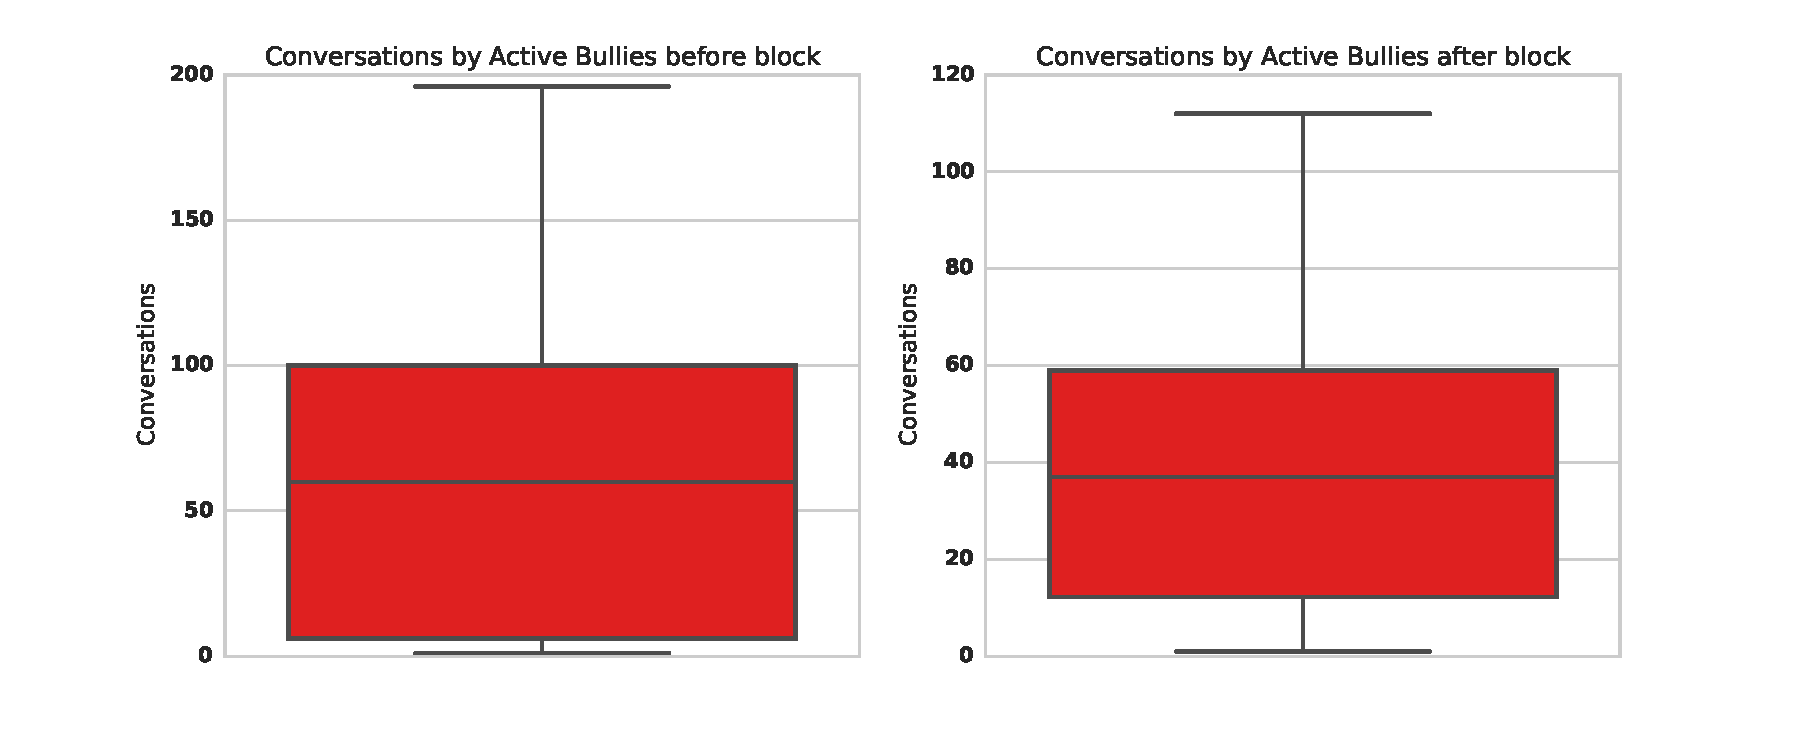
\includegraphics[width=5in]{B1.pdf} %include the saved image name in the braces as shown (VLSI_Chip.jpg)
	%%%% you can always adjust width of the image using command in square braces ([width=?in])
	\caption{Conversations of Bullies before and after block(s)} 
	\label{fig:4}
\end{figure}

\begin{figure}
	\centering %%%% this command is used to align center
	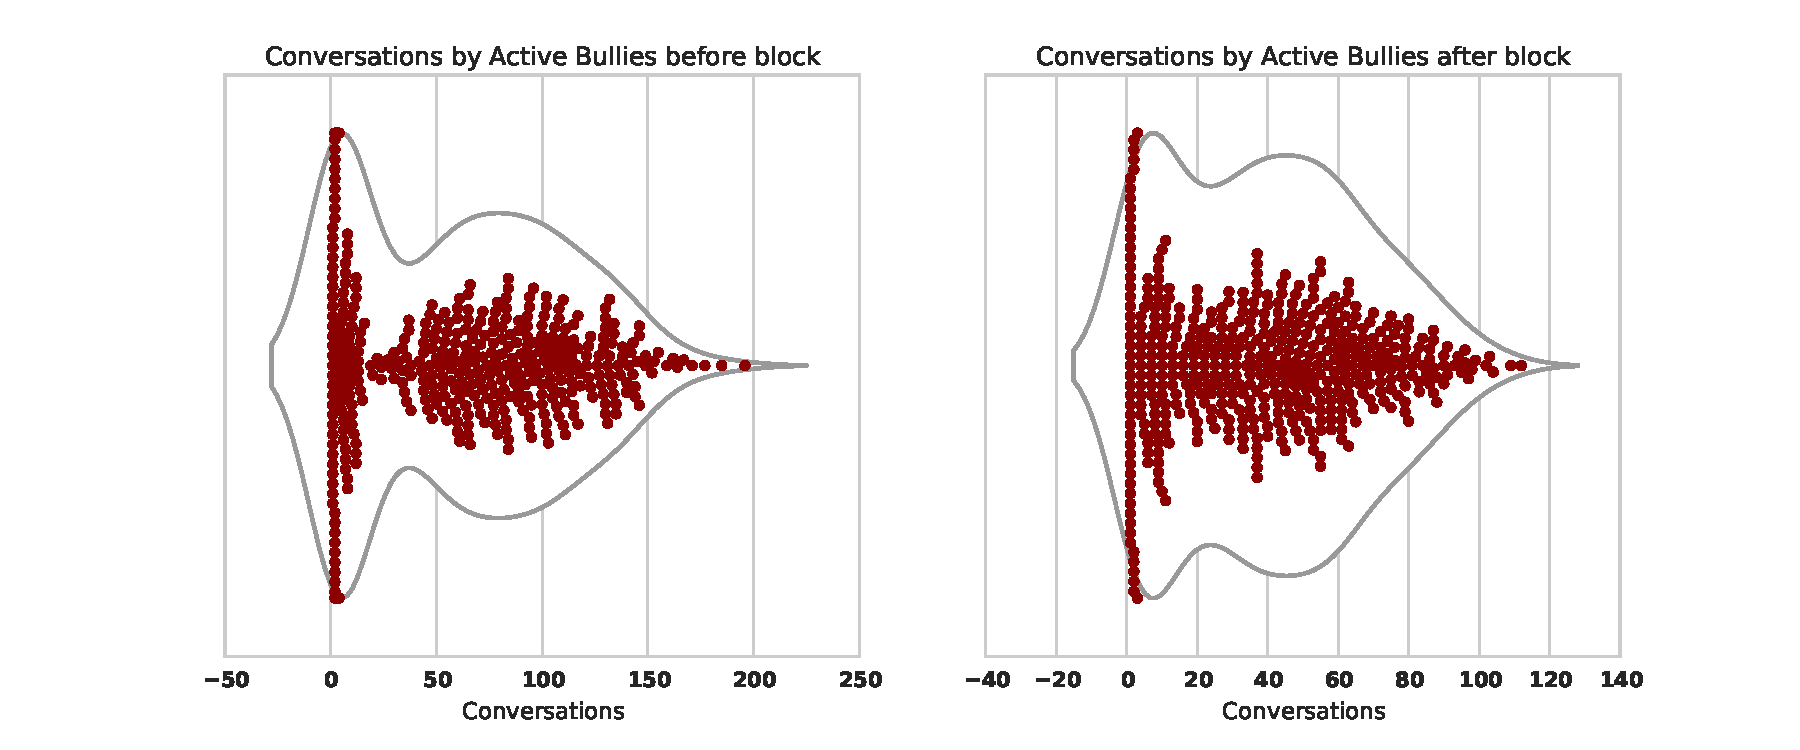
\includegraphics[width=5in]{v1.pdf} %include the saved image name in the braces as shown (VLSI_Chip.jpg)
	%%%% you can always adjust width of the image using command in square braces ([width=?in])
	\caption{Conversations of Bullies before and after block(s)} 
	\label{fig:5}
\end{figure}

\section{Summary of Findings}
The key takeaways from this chapter are as follows :
\begin{itemize}
\item Cyberbullying is the worst kind of evil born out of online social networks. No matter the online social system, cyberbullying should be expected to occur and 7cot is no exception.
\item Language analysis of the notes which are provided when a cyberbully is blocked revealed three distinct themes a cyberbully uses to harass the users, which are sexual harassment, rude behavior and trying to acquire personal information. Past research also revealed such themes for cyberbullying a user, so the themes of cyberbullying can be generalized into a few types. However, getting blocked for trying to acquire personal information looks unique on 7cot.
\item The standard measures adopted to thwart cyberbullying on the platform such as blocking or banning are effective. 
\end{itemize}
